\chapter{Spectral flow cytometry}
\label{chap:refs}

\section{Basic principles}
\label{subs:basic}
Flow cytometry is a method used to measure and quantify physical and biological properties of cells in a stream of fluid. 

For a cell sample to be processed by a \emph{cytometer}, cells must be prepared in single cell suspension. 

In a cytometer the cell suspension flows through a narrow tube known as a \emph{flow cell} or \emph{flow sheath}. 

Desirable flow of the sample fluid is achieved using \emph{hydrodynamic focusing}. This technique focuses the sample into a narrow stream using sheath fluid, generally allowing only one cell to pass at a time. This works thanks to principles established by fluid dynamics. When the two liquids differ enough in velocity or density they will not mix and instead create a stable layered flow\cite{HydrodynF2012}. 

A laser beam is then shone through the sample, captured using \emph{photon detectors} and the measured signal is amplified using photomultipliers: \cref{fig:cytm}.

\begin{figure}
  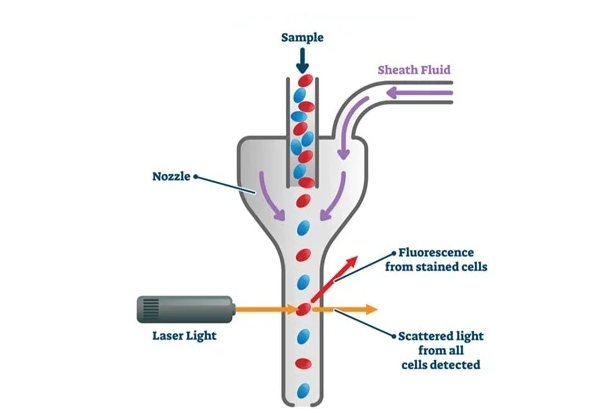
\includegraphics[width=0.9\linewidth]{img/hydro.png}
  \caption{Simplified flow cytometer schema[\url{https://www.shutterstock.com/}].}
  \label{fig:cytm}
\end{figure}

To estimate physical properties of the cell such as size and granularity we take advantage of \emph{light scattering} --- the phenomenon where photons are forced to change their direction by the medium they pass through\cite{scatter98}.

There are two types of scattering measured in cytometry \cref{fig:scatter}.

\emph{Forward scatter} - also referred to as \emph{FSC} or \emph{FSc},  refers to the light, with unchanged wavelength from the source, diffracted around the cell edges - this diffraction pattern roughly corresponds to the cells circumference. 

\emph{Side scatter} - also referred to as \emph{SSC} or \emph{SSc}, is a term used for the light scattered by the cell and its internal structures in the $\geq90^{\circ}$ angle --- this measurement serves as an approximation of cell granularity\cite{fundcyto2011bake}.
\begin{figure}
  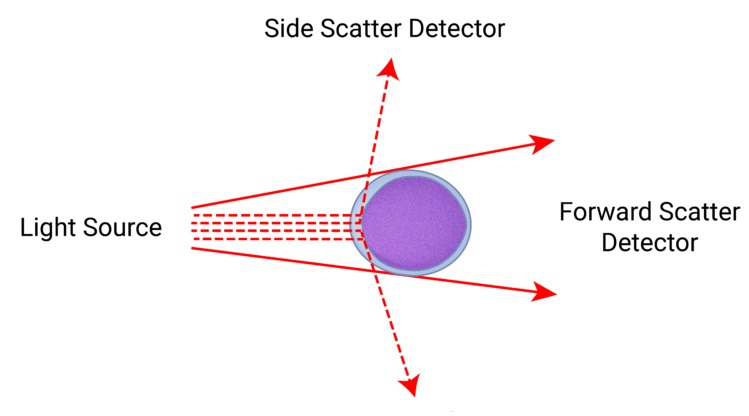
\includegraphics[width=0.65\linewidth]{img/ssc_fsc.jpg}
  \caption{Light scatter pattern for a cell in a cytometer[\url{https://www.learnhaem.com/courses/flow-cytometry/}]}
  \label{fig:scatter}
\end{figure}

In practice FSC and SSC can be used to distinguish cells of interest from cell debris and erythrocytes and furher distinguish broader cell types such as  lymphocytes, monocytes and granulocytes from each other: \cref{fig:gates} A. 

\begin{figure}
  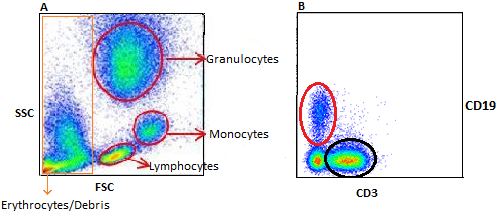
\includegraphics[width=0.75\linewidth]{img/gating.png}
  \caption{A) High-level cell type identification using FSC/SSC plot. B) Separating B (red) and T (black) cells using CD3/CD19 markers.}
  \label{fig:gates}
\end{figure}

To detect biological \emph{markers} such as proteins, we use \emph{antibodies} for the markers we wish to study and \emph{conjugate} them with a distinct \emph{fluorochrome}. 

For each \emph{fluorochrome} absorption and emission spectrum exists. 

Absorption spectrum is the wavelength range at which the fluorochrome can be excited, while the emission spectrum is the range at which it emits photons. 

The emitted light will always have longer wavelength than the absorbed light - this difference is called “Stokes shift”: \cref{fig:stokes}. Higher Stokes shift makes increases  the separation between excitation and emission spectrum easier.

In the context of this thesis, light of 320--808nm wavelength will be considered the main excitation source.

Conjugated antibodies bind to the marker of interest and since the bound fluorochrome emits a specific light spectrum when excited\footnote{\url{https://www.britannica.com/science/fluorescence}} this will alter the \emph{emission spectrum} of the cell.

Thanks to this process we can use a cytometer to measure the cell emission spectrum and later use computational methods and statistical analysis to \emph{unmix} and interpret the data which ultimately allows us to quantify the expression of the studied markers in our cell sample.

\Cref{fig:gates} B illustrates how a marker combination can be used to distinguish cell types and sub-types.

\begin{figure}
  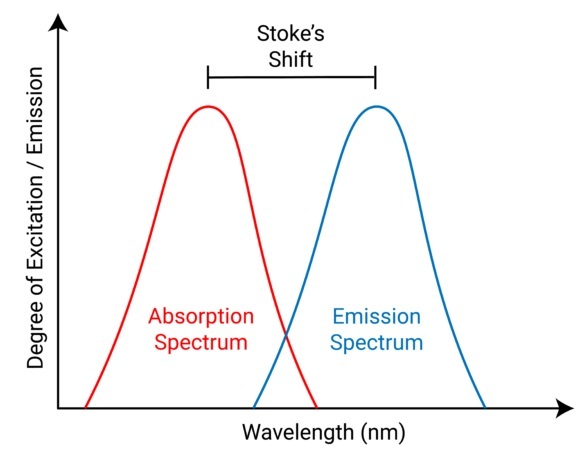
\includegraphics[width=0.5\linewidth]{img/stokes.jpg}
  \caption{Stokes shift [Image taken from Wikipedia article `Stokes shift']}
  \label{fig:stokes}
\end{figure}

It is also important to note that while a fluorochrome can be excited by a light source anywhere within its absorption spectrum, there is an optimal wavelength at which it will absorb the highest fraction of photons, maximizing subsequent emission. This wavelength is called maximal absorbance and the corresponding emission wavelength is called maximal emission. When excited outside of the maximal absorbance wavelength absorption efficiency is relatively decreased\footnote{\url{https://www.olympus-lifescience.com/en/microscope-resource/primer/lightandcolor/fluoroexcitation/}}.

The measured spectrum usually results from combination of the various bound conjugated antibodies and autofluorescence. We can also measure autofluorescence alone on unstained cells where no conjugated antibodies are present in the sample. 

In spectral flow cytometry we need to measure single stain controls - cells with just a single conjugated antibody bound, for every unique fluorochrome used in the current experiment. This is the source of the mixing matrix used for spectral unmixing\cite{mixmat}. 

Spectral flow cytometry leverages multiple lasers with different wavelengths and detector arrays to measure the entire spectrum across a specified wavelength range which is achieved by using a detector array with filters where every detector measures only a narrow part of the spectrum with typical band width of $5-50nm$ that passes through the appropriate filter.\cite{ctyoovw} 

This approach allows using many fluorochromes in a single experiment (up to $\sim 40$  color panels) in turn allowing for more complex cell profiling\cite{40OMIP2020}.

\section{Mixing and spillover}
\label{subs:mixing}

When measuring experiments using more than a few fluorochromes it is practically unavoidable for the respective emission spectra to overlap, meaning that multiple fluorochromes will activate the same detector for the same cell. This phenomenon is called \emph{spillover}.

The main drawback and challenge of spectral cytometry is the need to perform spectral unmixing to infer in what abundances were the fluorochromes originally mixed to produce the measured cell spectrum\cite{unmix2013nonsq}.
In a perfect world where the only noise we have to consider is gaussian and constant this seems to be a linear problem:
\begin{equation}
 y=Mx+r
 \label{eq:base}
\end{equation}

In \cref{eq:base} $y$ is the observation vector (measured spectrum) and $M=D \cdot f$ is a matrix of \emph{spectral signatures} for each of the fluorochromes used in the given experiment. $f$ represents rows of $M$ corresponding to unique fluorochromes used in the experiment while $D$ represents column corresponding to the detectors. $x$ is a vector of fluorochrome abundances and $r$ represents the discussed gaussian noise.\cite{unmix2013nonsq}

While the \emph{mixing matrix} $M$ is not known, it can be estimated using the single stain controls mentioned in \cref{subs:basic}. 

We assume that in any single experiment the number of detectors is higher than the number of fluorochromes, which typically holds true in the real world and leaves us with an overdetermined system of linear equations (more equations than unknowns) solution for which can be estimated using ordinary least-squares\cite{anton2005elementary}. 

A simplified practical example is outlined in \cref{chap:math}.

\section{Noise sources and characteristics}
There are multiple sources of noise in spectral flow cytometry such as staining related deviations, observed population inhomogeneity, electronic noise, noise originating from scattered light not properly excluded by the filters, dark current on photon detectors and noise from photon statistics - a stochastic process influencing both photon emission and detection \cite{noise1985}. 

Combination of the above factors makes the unmixing problem significantly more complicated than it might initially seem.

\subsection{Background noise}
Background noise can be characterized as combination of dark current, optical noise and electronic noise. Dark current is current flowing through a photon detector even without presence of photons. It is caused mainly by thermionic emission\cite{FlCytEl04}.
Optical noise is caused by stray light produced as a result of laser light scattering\cite{PosNoiseSteen92}.

Electronic noise can have many sources such as electromagnetic radiation produced by other electronic devices or other electronic components within the cytometer itself, heat and potentially even gamma rays and x-rays however, those are unlikely to be present in meaningful quantities.

Background noise is relatively independent on current signal. Since it is somewhat constant and relatively low, it can be measured and thresholded against minimizing its impact\cite{FlCytEl04}.
\subsection{Autofluorescence}
Autofluorescence acts as another source of noise with characteristics dependent on the particular cell. It is caused by various compounds and structures inside the cell, such as collagen, elastin, cyclic compounds (commonly pyridine nucleotides) and flavins \cite{af1}\cite{af2}. In mammalian cells the typical excitation range for aurofluorescence lies between 375 to $\sim$640 nm and its typical emission range between $\sim$400 to $\sim$700+ nm\cite{af_ranges}. 

Autofluorescence can be used for unmixing as another spectrum in the mixing matrix $M$, as well as subtracted from the single stain control spectra and the spectra of measured cells prior to unmixing\footnote{\url{https://www.thermofisher.com/cz/en/home/life-science/cell-analysis/flow-cytometry/flow-cytometry-learning-center/flow-cytometry-resource-library/flow-cytometry-methods/spectral-flow-cytometry-fundamentals.html}}. 


When accounted for in unmixing we are effectively negating the noise coming from varition in Autofluorescence strength --- if one cell has 2$\times$ the amount of Autofluorescence as another this is no longer noise instead it becomes an abundance for the Autofluorescence spectrum for that cell in the unmixed data. This effectively helps us lower the amount of noise from Autofluorescence that remains in the data. It now only stems from variations in the shape of Autofluorescence spectrum for individual cells but no longer from its intensity\footnotemark[3]. 

\newpage
\subsection{Poisson (shot) noise}
Poissonian characteristics of photon emission are given by the particle-like nature of light.
The quanta representing photon particles fluctuate in time and these fluctuations can only have discrete values.
This process is best modelled using Poisson distribution function where $\lambda$ is the expected value for number of emitted photons per unit of time\cite{MandelPoisStat1959}.
\begin{figure}
  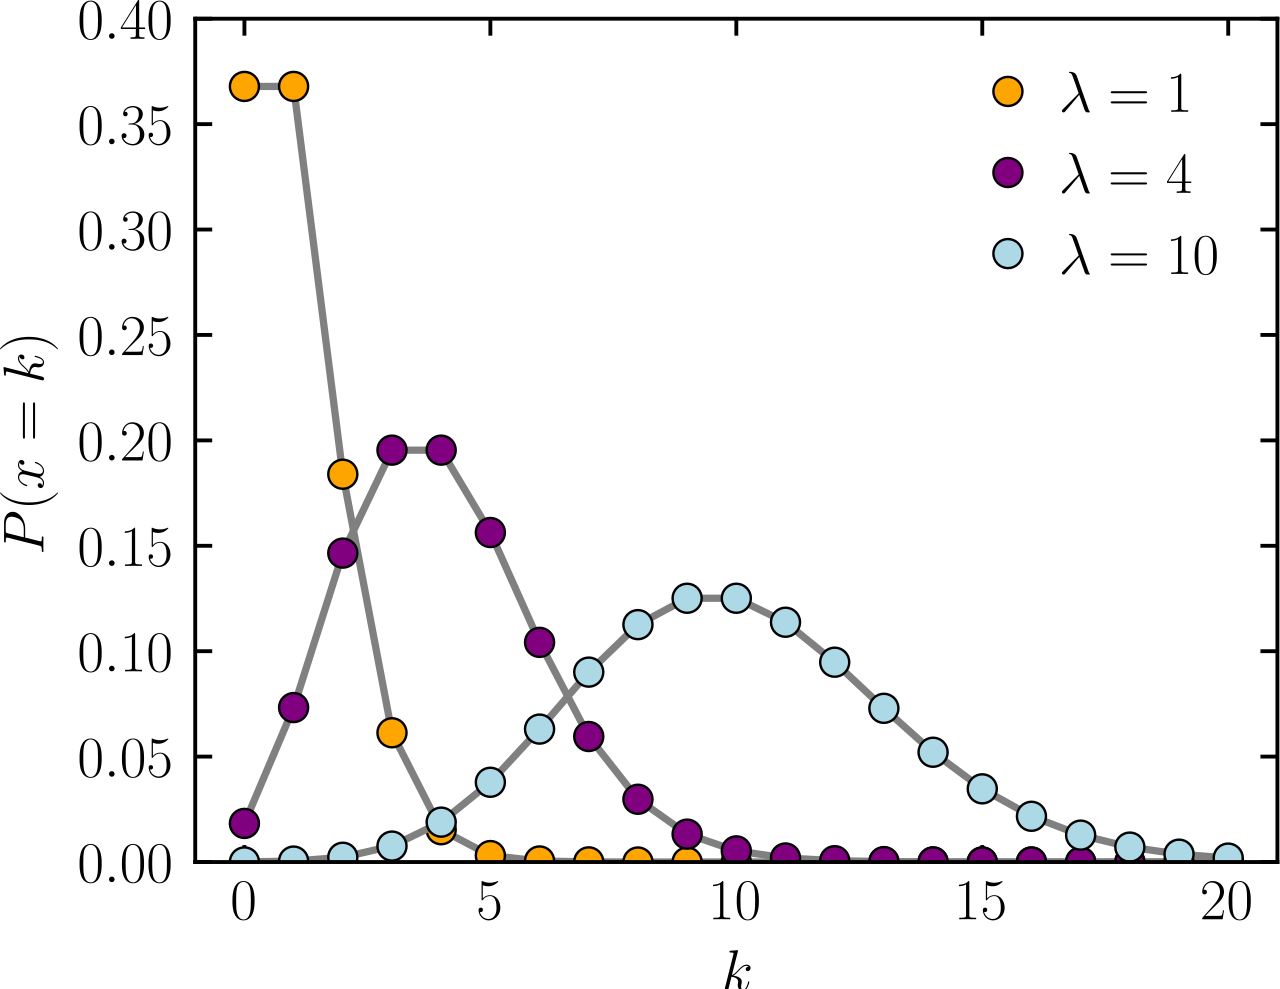
\includegraphics[width=0.7\linewidth]{img/poisson.png}
  \caption{Poisson probability distribution($\lambda=(1,4,10)$) [From Wikipedia.com article `Poisson distribution'].}
  \label{fig:pois}
\end{figure}
 With increasing $\lambda$ the Poisson distribution becomes more and more similar to binomial distribution eventually approximating continuous gamma distribution and finally with high enough $\lambda$ we can say that Poisson distribution approximates normal distribution as seen in \cref{fig:pois}.

There are multiple sources of Poisson noise in spectral flow cytometry:
\begin{itemize}
    \item \emph{Bias light shot noise}
    
    Poissonian noise resulting from background light - this noise should be independent of the current signal level however, it is dependent on the particular optical system (cytometer)\cite{PosNoiseSteen92}. 
    It can also be considered a part of background noise for simplicity.
    
    Assuming that the optical system is in a relatively stable and controlled environment this noise should be constant and can be thresholded against as a part of background noise.
    
    \item \emph{Expression and luminance based noise}
    
    Expression based noise dependens on total expression of targeted proteins by the measured cell. 
    The more targets are expressed, the more conjugated antibodies are going to bind inside the cell. This in turn leads to more internal light scattering, diffraction and interference resulting in higher noise\cite{noise1985}. This noise is unavoidable on real cells that express any of the targets.
    
    Luminance based noise depends on the magnitude of the fluorescent light or fluorescent power --- the integral of the measured cell spectrum. This noise increases across all detectors with rising total fluorescent power making it more significant in dim and less significant in bright detectors\cite{PosNoiseSteen92}. 
    Since this is the signal we want to measure it is also unavoidable. 
\end{itemize}